\chapter{Implementing the System: The Back-End}
	\label{chap:impl:backend}
	In chapter \ref{chap:design} the design of the solution was described. This description ranged from overall specifications, to more detailed model designs. In the following two chapters the implementation of a \emph{prototype}, following the design specifications from chapter \ref{chap:design}.

	To achieve the best possibly experience for the reader, the description is split into two parts: The back-end and the front-end. In \emph{this} chapter, the implemenation of the prototype back-end is described.


	\section{The Language of the Back-End}
		When developing a REST back-end, there exists numerous tools for the job. Amongst others, are
		\begin{itemize}
			\item Python
			\item Node.js
			\item PHP
		\end{itemize}
		While this list is \emph{by far} complete, it more or less states the most popular options for REST APIs and web applications, these days.

		\subsection{Python}
			One of the more popular languages for self-hosted software is Python. Python requires what is called Web Server Gateway Interface \emph{(WSGI)} server, to be able to run a webservice. Common implementations of such a server, is Django and Flask. Part of the popularity of Python is most likely the ease of which it is read. The Raspberry Pi foundation \emph{specifically} states, that:
			\begin{citequote}{rpi_python}
				Python is a wonderful and powerful programming language that's easy to use (easy to read and write).
			\end{citequote}

			 Amongst others, PayPal uses Python for their services.

		\subsection{Node.js}
			In the later years, node.js has become more and more widespread. This is partly due to how it \emph{very} effectively handles multiple requests. While ``traditional'' sequential languages -- like python -- would spawn a thread per request, Node.js uses asynchronous code and is centered around non-blocking I/O. As such, while node strictly speaking only ever uses one thread, it can handle \emph{massive} amounts of traffic quite easily. However, this does change the programming style of Node.js programs, as it uses callback methods and JavaScript promises to a large extent. Additionally, Node.js is built ontop of Google's V8 engine, and supports C++ plugins, should it be necessary.

			One of the development advantages to nodejs, is that it uses Javascript. Most web applications these days use JavaScript, and being able to code the back-end in the same language, might very well make it easier for a developer to quickly move between front-end and back-end.

		\subsection{PHP}
			PHP is without a doubt the most widespread language used for server-side scripting, when it comes to websites. However, this language can also be used to actually develop a REST api. While previously PHP would have to be executed on top of an Apache server or nginx server, in newer versions PHP support a native web-server. While this, strictly speaking, is only intended for development purposes, there is nothing stopping you from running a small-scale service using this server.

		\subsection{Making A Choice}
			Taking the various options into consideration, it is concluded that the back-end will be developed using Node.js. This choice is greatly influenced by the fact that it would share development language with the front-end, thus making venturing into new territory slightly less daunting.

	\section{To Framework or Not To Framework}
		Having decided to go with Node.js for the back-end, the next big question arises: To framework or not to framework? Node.js has its own built-in webserver, and it is perfectly viable to simply use this. However, using frameworks will inevitably make it \emph{easier} to code. As such, it is decided that a framework will be used, to aid the development of the back-end.

		When it comes to these frameworks, there is no doubt that Express is the ``biggest'' one: It is simply the most widespread and popular of the frameworks available. However, alternatives such as Restify, Hapi, and Koa also exist. While these four by no means constitute the entire list of frameworks, they are the four largest.



		\subsection{Express}
		\subsection{Hapi}
		\subsection{Restify}
		\subsection{Koa}

	\section{Node.js Coding Style}
		When developing using node.js there are two different schools of thought: Callbacks and promises. Since node.js asynchronous, traditional synchronous methods should not be used. For reference purposes, the \emph{wrong} way to do it, is shown on figure \ref{lst:node:wrong}. This causes major performance issues, as the execution of the program would halt, while the action taking a long time is performed.

		On listing \ref{lst:node:callback} on page \pageref{lst:node:callback}, the same output is shown using callbacks. When the data that takes a long time to produce, or fetch, is ready, the callback is called, with the result. As such, while the I/O is happening the node thread can continue working.

		Finally, there is listing \ref{lst:node:promise} on page \pageref{lst:node:callback}. This example uses promises, to achieve the same thing. By many, promises are thought to be the successor of callbacks. Some of the internals of the promise based method have been omitted, such as the proper use of deferreds, as this is beyond the point of this section.

		Conceptually promises are by \emph{far} the harder of the two to understand. Using them properly, without creating unnecessary overhead takes some getting used to. \emph{However} they do produce code which is \emph{much} easier to read. This is in partial due to what is commonly called ``promise chaining''. Essentially, this takes the output from one promise, and pipes it to the input for another function. 

		The above is best described using an example. In this scenario, there are three methods: \verb=fetch=, \verb=compute=, and \verb=send=, which are to be executed in that order. \verb=fetch= fetches the data from a remote source, \verb=compute= does some computations on said data, and finally \verb=send= sends the result of said computations somewhere else. On listing \ref{lst:node:callbackhell} on page \pageref{lst:node:callbackhell} this sequence of events are shown, using callbacks. As seen, the cascade of callbacks make this code \emph{horrible} to read. Professionals often use the derogatory term ``callback hell'', to describe this phenomenon. On listing \ref{lst:node:promisegoodness} on page \pageref{lst:node:promisegoodness} this \emph{exact} same sequence of events is shown, only using promises. As it is seen, this code is \emph{much} easier to read and understand. As such, using promises for this solution is by far preferable and is the style that will be used, whenever possible.


		\begin{lstlisting}[language=Javascript,gobble=12,caption={Using callbacks, in Node.js},label={lst:node:callback}]
            function longTime(callback){
                // Something that takes a loooong time
                var res = ...
                callback(res);
            }
            
            longTime(function(r){
                console.log(r);
            });
		\end{lstlisting}

		\begin{lstlisting}[language=Javascript,gobble=12,caption={Using promises, in Node.js},label={lst:node:promise}]
            function longTime(){
                var deferred = Promise.defer();
                // Something that takes a loooong time
                var res = ...
                return deferred;
            }
            
            longTime()
            .then(function(r){
                console.log(r);
            })
		\end{lstlisting}

		\begin{lstlisting}[language=Javascript,gobble=12,caption={The wrong way to do it, in Node.js},label={lst:node:wrong}]
            function longTime(){
                // Something that takes a loooong time
                var res = ...
                return res;
            }
            console.log(longTime());
		\end{lstlisting}
		

		\begin{lstlisting}[language=Javascript,gobble=12,caption={Chaining data between callbacks in node.js},label={lst:node:callbackhell}]
            get(function(data){
                compute(data, function(newData){
                    send(newData, function(){
                        console.log("Done!");
                    })
                })
            })
		\end{lstlisting}
		
		\begin{lstlisting}[language=Javascript,gobble=12,caption={Chaining data between promises in node.js},label={lst:node:promisegoodness}]
            get()
            .then(compute)
            .then(send)
            .then(function(){
                console.log("Done!");
            })
		\end{lstlisting}

	\section{Structuring the Codebase}
		When it comes to a codebase's readability and maintainability, a good structure is almost the most important thing. As such, a proper categorisation is the first thing needed. Fundamentally, there will be four different types of code files, in the project: Models, routes, tests, and middleware.

		Models represent on-disk data structures, as will be stored in the database. These were covered in section \ref{sec:moddeling} on page \pageref{sec:moddeling}. Since node.js natively supports ECMAScript 6 objects, these models will be represented as objects in memory. The models also contains the relevant methods for manipulating the entries. An example of this could be looking up a user, from an ID.

		Routes represent API endpoints. These are described in full detail, in section \ref{sec:impl:api} on page \pageref{sec:impl:api}. These routes will be separated into files representing their primary resource.

		Tests should hopefully be obvious. These are the unittests for the back-end. Further details regarding testing framework and methodology is found in section \ref{sec:impl:tests} on page \pageref{sec:impl:tests}.

		Middleware would be the last category. What exactly these are, is explained in further details in section \ref{sec:impl:middleware} on page \pageref{sec:impl:middleware}.

		As such, the basic structure of the back-ends codebase will be as follows:
		\dirtree{%
		.1 project.
		.2 app.js
		.2 middlewares.
		.2 models.
		.2 routes.
		.2 tests.
		}
	\section{Database Abstraction Layer}
		As decided in section \ref{sec:restrict:database} on page \pageref{sec:restrict:database}, a database abstraction layer is necessary. While Object-Relational Mapping \emph{(ORM)} strictly speaking isn't the same as a DAL, for this section the two are considered equivalent.

		The two most widely used solutions for this, is Sequelize, Bookshelf, and Knex \emph{(Bookshelf is built ontop of Knex)}. Sequelize and Bookshelf are both ORMs, whereas Knex is a DAL. In regards to platform support, they are fairly similar. Sequelize supports PostgreSQL, MySQL, SQLite and MSSQL. Bookshelf/Knex supports MySQL, SQLite, Postgres, MariaDB, and Oracle.

		While working with ORMs generally takes database interactions to a higher abstraction level, it is thought that this also removes certain insight into how some queries work. Additionally, Knex's chainable methods, makes for query building in the style of Javascript promises. As such, it is concluded the Knex is the superior choice as a DAL for the implementation.

	\section{API Endpoints}
		\label{sec:api}
		Before defining the endpoints, the resources \emph{(see section \ref{sec:design:rest} on page \pageref{sec:design:rest})} of the application need to be determined. Looking at the models defined in section \ref{sec:modelling} on page \pageref{sec:modelling}, these offer a great starting point for resources.

		\subsection{The Users Resource}
			First and foremost there is the collection of Users. This collections represents the user base as a whole. \verb=POST=ing to this collection, would by extension mean the creation of a new user. \verb=GET=ing the user collection, mean retrieving all user entries, with their username and other attributes in the ``public domain''. \verb=PUT= and \verb=DELETE= is slightly different. They're used for updating and deleting a \emph{single} user, in the entire collection. As such, the endpoint needs to have a user ID postfixed. Adhering to the standard, \emph{all} API endpoints will have \verb=/api= prefixed. These API endpoints are listed on table \ref{tab:api:users} on page \pageref{tab:api:users}.

		\subsection{The Passwords Resource}
			Then there is the collection of passwords. However, there is a slight caveat when it comes to this collection. Since each password is \emph{owned} by a user, it can generally be thought that there exists \emph{multiple} collection -- one for each user. As such, the password collection is gated behind the user resource and the ID specifying exactly which user owns said password. The same approach to designing these endpoints are used, as with the user resource and the result of this is found on table \ref{tab:api:passwords} on page \pageref{tab:api:passwords}.

			For simplicity's sake, access to shared passwords are gated behind the passwords resource. As such, a collection called shares -- which belongs to a specific password -- denotes the collection of users this specific password has been shared to. Additionally, two collections are added as well: \verb=shared= and \verb=shares=. These two are  \emph{very} similar in name, which unfortunately might result in some confusion. The \verb=shares= resource denotes passwords shared \emph{to} the user and the \verb=shared= resource denotes passwords that the user has shared to \emph{others}. These endpoints are found on table \ref{tab:api:sharedpasswords} on page \pageref{tab:api:sharedpasswords}.

		\subsection{The Categories Resource}
			The same argument made in regards to the passwords collection, can be said about categories. Each user has their own private password collection, which is -- similar to passwords -- gated behind the owning user's ID. This can be seen on table \ref{tab:api:categories} on page \pageref{tab:api:categories}.

		\subsection{The Invites Resource}
			When an admin creates a new invites, it can be said he \verb=POST=s it to the invites resource. \verb=GET=ing an ID, returns the status of an ID stored in the database. Then, there is finally the act of using an invite. Since a user is created, it only makes sense that the \verb=POST= method is needed. However, since the regular endpoint is already being posted to, an additional endpoint is needed. As such, appending the endpoint with \verb=/accept= will achieve this. This can be seen on table \ref{tab:api:invites} on page \pageref{tab:api:invites}.

		\subsection{The Audit Resource}
			The Audit resource is actually very simple. It only consists of a single endpoint; Getting the audit log. Since this resource is owned by individual users, this is -- much like passwords and categories -- gated behind the user collection and a specific ID. This can be seen on table \ref{tab:api:audit} on page \pageref{tab:api:audit}.

		\subsection{The Auth Resource}
			\label{sec:api:auth}
			The Auth resource is a little bit more interesting. Of course, there is the generic \verb=POST=, containing the user's username and password, for authentication purposes. The details of this is covered in section \ref{sec:design:authentication} on page \pageref{sec:design:authentication}. However, this is not all. Since the solution supports TOTP two-factor-authentication, as described in section \ref{sec:mfa} on page \pageref{sec:mfa}, endpoints for enabling this is needed as well. In section \ref{sec:design:breaking-rest} on page \pageref{sec:design:breaking-rest} it was argued that at one point it was \emph{necessary} to break the REST principles. As such, two endpoints are needed: One for generating a new secret and caching it, and one for actually verifying said secret. 


		
		\newcolumntype{L}[1]{>{\hsize=#1\hsize\raggedright\arraybackslash}X}%
		\newcolumntype{R}[1]{>{\hsize=#1\hsize\raggedleft\arraybackslash}X}%
		\newcolumntype{C}[2]{>{\hsize=#1\hsize\columncolor{#2}\centering\arraybackslash}X}%
		
		\begin{table}
			\definecolor{tablerow1}{RGB}{230,230,230}
			\definecolor{tablerow2}{RGB}{255,255,255}
			\rowcolors{2}{tablerow1}{tablerow2}
			
			\begin{tabularx}{\textwidth}{ R{0.15} | L{0.65} | L{0.2} }
				\bfseries Method & \bfseries Endpoint & \bfseries Description% specify table head
				\csvreader[head to column names]{resources/api/users.csv}{}% use head of csv as column names
				{\\\hline\method & \texttt{\endpoint} & \description}% specify your coloumns here
			\end{tabularx}

			\caption{API endpoints for the Users resource.}
			\label{tab:api:users}
		\end{table}


		\begin{table}
			\definecolor{tablerow1}{RGB}{230,230,230}
			\definecolor{tablerow2}{RGB}{255,255,255}
			\rowcolors{2}{tablerow1}{tablerow2}
			
			\begin{tabularx}{\textwidth}{ R{0.15} | L{0.65} | L{0.2} }
				\bfseries Method & \bfseries Endpoint & \bfseries Description% specify table head
				\csvreader[head to column names]{resources/api/passwords.csv}{}% use head of csv as column names
				{\\\hline\method & \texttt{\endpoint} & \description}% specify your coloumns here
			\end{tabularx}

			\caption{API endpoints for the Passwords resource.}
			\label{tab:api:passwords}
		\end{table}

		\begin{table}
			\definecolor{tablerow1}{RGB}{230,230,230}
			\definecolor{tablerow2}{RGB}{255,255,255}
			\rowcolors{2}{tablerow1}{tablerow2}
			
			\begin{tabularx}{\textwidth}{ R{0.15} | L{0.65} | L{0.2} }
				\bfseries Method & \bfseries Endpoint & \bfseries Description% specify table head
				\csvreader[head to column names]{resources/api/sharedPasswords.csv}{}% use head of csv as column names
				{\\\hline\method & \texttt{\endpoint} & \description}% specify your coloumns here
			\end{tabularx}

			\caption{API endpoints for accessing Shared Passwords.}
			\label{tab:api:sharedpasswords}
		\end{table}		

		\begin{table}
			\definecolor{tablerow1}{RGB}{230,230,230}
			\definecolor{tablerow2}{RGB}{255,255,255}
			\rowcolors{2}{tablerow1}{tablerow2}
			
			\begin{tabularx}{\textwidth}{ R{0.15} | L{0.65} | L{0.2} }
				\bfseries Method & \bfseries Endpoint & \bfseries Description% specify table head
				\csvreader[head to column names]{resources/api/categories.csv}{}% use head of csv as column names
				{\\\hline\method & \texttt{\endpoint} & \description}% specify your coloumns here
			\end{tabularx}

			\caption{API endpoints for the Categories resource.}
			\label{tab:api:categories}
		\end{table}
		
		\begin{table}
			\definecolor{tablerow1}{RGB}{230,230,230}
			\definecolor{tablerow2}{RGB}{255,255,255}
			\rowcolors{2}{tablerow1}{tablerow2}
			
			\begin{tabularx}{\textwidth}{ R{0.15} | L{0.65} | L{0.2} }
				\bfseries Method & \bfseries Endpoint & \bfseries Description% specify table head
				\csvreader[head to column names]{resources/api/invites.csv}{}% use head of csv as column names
				{\\\hline\method & \texttt{\endpoint} & \description}% specify your coloumns here
			\end{tabularx}

			\caption{API endpoints for the Invites resource.}
			\label{tab:api:invites}
		\end{table}

		\begin{table}
			\definecolor{tablerow1}{RGB}{230,230,230}
			\definecolor{tablerow2}{RGB}{255,255,255}
			\rowcolors{2}{tablerow1}{tablerow2}
			
			\begin{tabularx}{\textwidth}{ R{0.15} | L{0.65} | L{0.2} }
				\bfseries Method & \bfseries Endpoint & \bfseries Description% specify table head
				\csvreader[head to column names]{resources/api/audit.csv}{}% use head of csv as column names
				{\\\hline\method & \texttt{\endpoint} & \description}% specify your coloumns here
			\end{tabularx}

			\caption{API endpoint for the Audit resource.}
			\label{tab:api:audit}
		\end{table}

		\begin{table}[p]
			\definecolor{tablerow1}{RGB}{230,230,230}
			\definecolor{tablerow2}{RGB}{255,255,255}
			\rowcolors{2}{tablerow1}{tablerow2}
			
			\begin{tabularx}{\textwidth}{ R{0.15} | L{0.65} | L{0.2} }
				\bfseries Method & \bfseries Endpoint & \bfseries Description% specify table head
				\csvreader[head to column names]{resources/api/auth.csv}{}% use head of csv as column names
				{\\\hline\method & \texttt{\endpoint} & \description}% specify your coloumns here
			\end{tabularx}

			\caption{API endpoints for the Auth resource.}
			\label{tab:api:auth}
		\end{table}

	\section{Workaround To Be Self-Contained}
		Unfortunatly, Restify's documentation is sometimes lackluster. They have what they call the serveStatic method. From their decription, its intended use is to deliver a default file, if a match is not found. This is exactly what is needed for the front-end's router \emph{(more on this in section \ref{sec:impl:ui-router} on page \pageref{sec:impl:ui-router})}. However, after much fiddling, it was found simply not to work.

		As such, a workaround is needed. After having stated the API routes, six new routes are defined as is seen on table \ref{tab:api:workaround} on page \pageref{tab:api:workaround}. This ensures that any API hits are given the proper error code, while ensuring that the application for the front-end is being delivered in all cases.
		\begin{table}
			\centering
			\begin{tabular}{r | l}
				\textbf{Method} & \textbf{Endpoint} \\
				\hline
				\verb=GET=		& \verb=/api/.*= \\
				\verb=HEAD=		& \verb=/api/.*= \\	
				\verb=POST=		& \verb=/api/.*= \\	
				\verb=PUT=		& \verb=/api/.*= \\
				\verb=DEL=		& \verb=/api/.*= \\
				\verb=PATCH=	& \verb=/api/.*= \\	
			\end{tabular}
			\caption{Workaround error routes, to make the API adhere to standards and the front-end's router to work \emph{(see section \ref{sec:impl:ui-router} on page \pageref{sec:impl:ui-router})}}
			\label{tab:api:workaround}
		\end{table}
		%RESTIFY workaround with serve static

	\section{Validating Input}
		\todo{Write about use of schemagic}

	\section{Middlewares}
		\label{sec:impl:middleware}
		To ease implementation and to reduce code duplication, certain features will be implemented using what is commonly known as middlewares. Middlewares are simply a term for methods, being executed \emph{before} the actual controller of an endpoint. An example of an endpoint is:
		\begin{lstlisting}[gobble=12,language=JavaScript]
            server.get('/api/ping', function(req, res, next){
                res.send(200, 'OK');
                return next();
            });		
		\end{lstlisting}

		Whenever \emph{any} client performs a HTTP call to the endpoint \verb=/api/ping=, using the \verb=GET= method, the server simply returns http code \verb=200=, and continues its operation. However, a new middleware will now be created. This middleware will effectively \emph{log} whenever a ping request is made. The code for the logger is found on listing \ref{lst:example:pinglog} on page \pageref{lst:example:pinglog}. Listing \ref{lst:example:ping_wlog} on page \pageref{lst:example:ping_wlog} now contains the updated ping endpoint. As is seen on line 2, the variable \verb=pinglog= is injected into the controller. As such, the code on listing \ref{lst:example:pinglog} is executed \emph{before} the code from listing \ref{lst:example:ping_wlog}, \emph{every} single time.

		\begin{lstlisting}[gobble=12,language=JavaScript,caption={PingLog Middleware},label={lst:example:pinglog}]
            module.exposts = function(req, res, next){
                console.log('Ping reqeuest received');
                return next();
            }
		\end{lstlisting}

		\begin{lstlisting}[gobble=12,language=JavaScript,caption={Ping endpoint with the pinglog middleware},numbers=left,label={lst:example:ping_wlog}]
            var pinglog = require('pinglog.js');
            server.get('/api/ping', pinglog, function(req, res, next){
                res.send(200, 'OK');
                return next();
            });		
		\end{lstlisting}

		This design approach is used for several features in the codebase, most noticibly:
		\begin{itemize}
			\item Authentication \emph{(see section \ref{sec:impl:authentication} on page \pageref{sec:impl:authentication})}
			\item Authorization \emph{(see section \ref{sec:impl:authorization} on page \pageref{sec:impl:authorization})}
			\item Object Resolving \emph{(see section \ref{sec:impl:resolve} on page \pageref{sec:impl:resolve})}
		\end{itemize}

	\section{Authentication}
		\label{sec:impl:authentication}
		In section \ref{sec:api:auth} on page \pageref{sec:api:auth} the endpoints involved in authentication was described. In this section, the process is described a little further. 

		As with any authentication, the user starts by sending his or her username and password \emph{(see section \ref{sec:design:authentication} on page \pageref{sec:design:authentication})}. If two factor authentication is not enabled, the standard verification approach is made. If the password matches, http code \verb=200= is returned, signifying successful authentication. Should it not match, http code \verb=401= is returned, signifying unsuccessful authentication. All in all, very basic.

		Should two factor authentication be enabled, however, a more complex event happens. Since the front-end won't know if two factor authentication is enabled or not, this needs to be conveyed to the front-end. As such, should the user have two-factor authentication enabled, but the token is missing from the body, http error code \verb=403= is returned. \verb=403= is defined as follows, by RFC2616\cite{httpcodes}:
		\begin{citequote}[sec.10.4.4]{httpcodes}
			   The server understood the request, but is refusing to fulfill it...
		\end{citequote}
		When the front-end receives the \verb=403= from the authentication endpoint, it \emph{knows} to promt to the user for a two-factor-token. Once this token is obtained, the request is sent again -- with the new token. Once received, the back-end verifies the password, similar to before, and verifies that the token is correct. If all fields are vitrified the back-end responds with \verb=200= to signify successful authentication. Should both fields not be verified, the response is \verb=401= to signify unsuccessful authentication. Figure \ref{fig:sequence:auth} on page \pageref{fig:sequence:auth} depicts this series of event, in a sequence diagram.

		\begin{figure}[p]
			\centering
			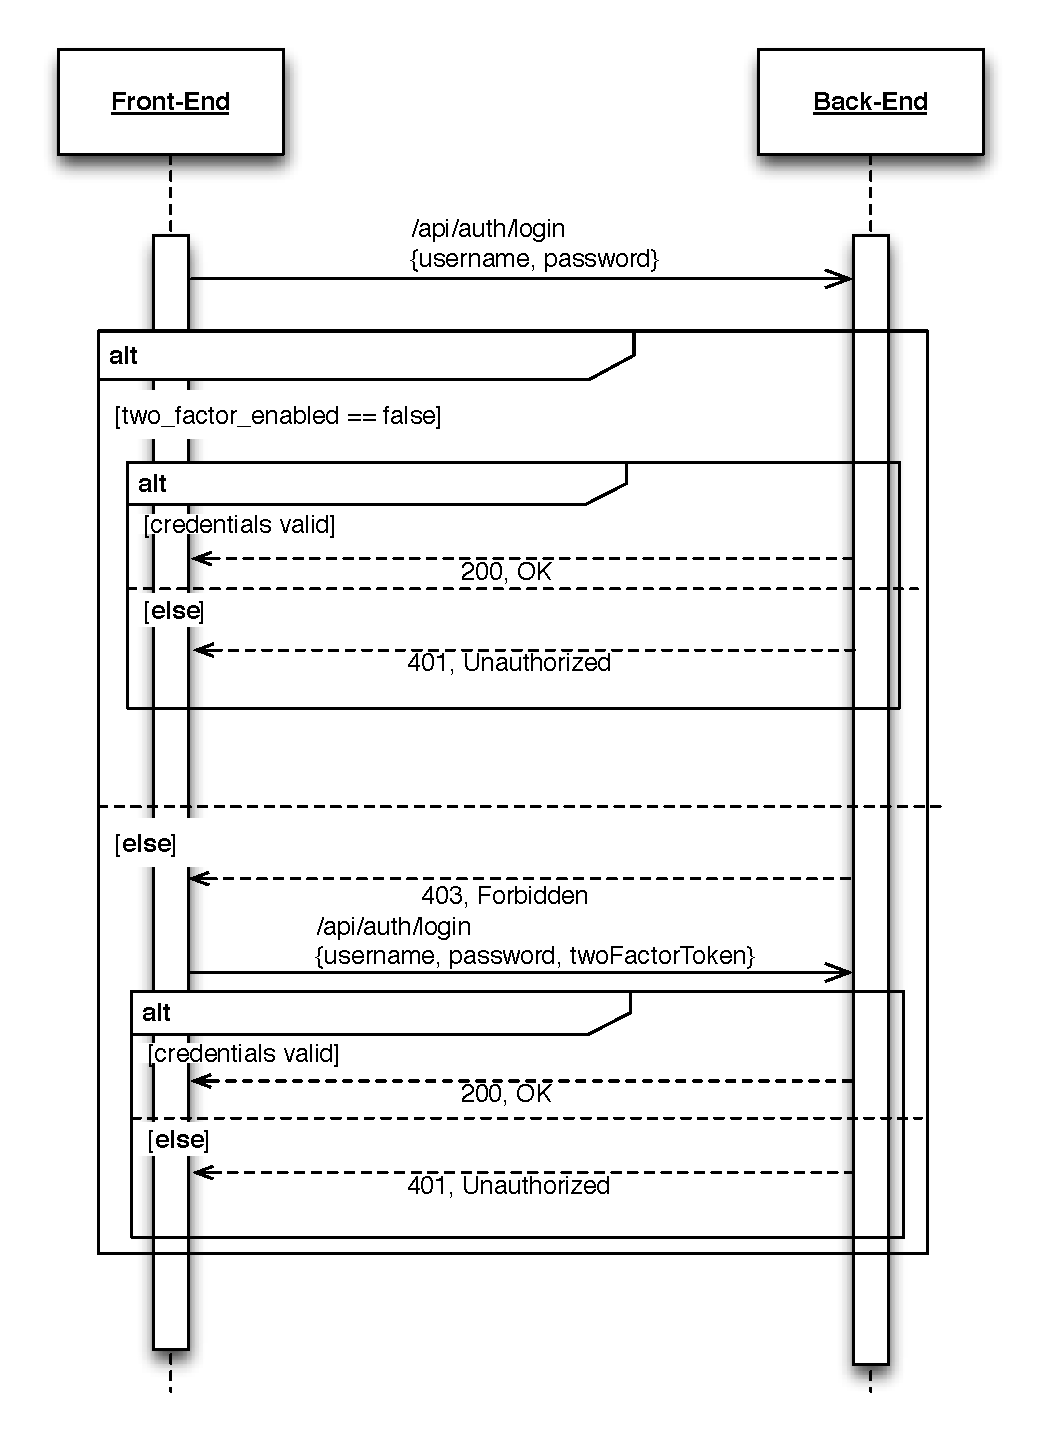
\includegraphics[width=0.8\textwidth]{figures/implementation/uml/sequence/authentication.eps}
			\caption{Sequence diagram showing the process of how the front-end authenticates to the back-end.}
			\label{fig:sequence:auth}
		\end{figure}

		\subsection{Powering the Two-Factor Authentication}
			To aid in the development, a third party tool is chosen for aiding the two-factor authentication. The Speakeasy project\cite{speakeasy_lib} is not only well documented and extremely easy to use, it is also pretty much the only two-factor authentication tool for Node.js, that has any credibility at all. As such, the choice fell on this suite.

			Speakeasy not only makes appropriate TOTP secret generation easy, but also makes verifying a token extremely easy. The snippet for verification is found on listing \ref{lst:example:speakeasy:verification} on page \pageref{lst:example:speakeasy:verification} \emph{(example taken from their GitHub repository)}. \verb=base32secret= is the secret that the TOTP client and the back-end has in common, and \verb=userToken= is the TOTP token.


			\begin{lstlisting}[gobble=16,language=JavaScript,caption={Verifying a TOTP token using Speakeasy},label={lst:example:speakeasy:verification}]
                var verified = speakeasy.totp.verify({ secret: base32secret, encoding: 'base32', token: userToken });
			\end{lstlisting}

	\section{Authorization}
		\label{sec:impl:authorization}
		For authorization purposes two strategies will be used: Simple and advanced. For all purposes where the simple is a possibility, it will be used. In section \ref{sec:design:authorization} on page \pageref{sec:design:authorization} it was described which users has access to which entities. The following two sections will adhere to this design.

		\subsection{Basic Authorization}
			Using the API described in section \ref{sec:api} on page \pageref{sec:api}, it is clearly seen that models' IDs are found in the URL. As such, using the owner field, of these models, it can easily be determined if the authenticated user has access to any given resource.

			As per the design, \emph{both} the user and admins will have full access to all user methods. This is simply handled with a comparison:
			\begin{lstlisting}[gobble=16,language=JavaScript]
                if( req.resolved.user.id === user.id || req.resolved.user.isAdmin ){
			\end{lstlisting}

			Since it is only the user self, that has access to his or her passwords, this is also handled extremely easy by doing:
			\begin{lstlisting}[gobble=16,language=JavaScript]
                if( password.owner === user.id && user.id === req.resolved.user.id ){
			\end{lstlisting}
			The exact same is done for categories:
			\begin{lstlisting}[gobble=16,language=JavaScript]
                if( category.owner === user.id && user.id === req.resolved.user.id ){
			\end{lstlisting}

			Shared passwords however, are a little bit more difficult. As has already been stated, both the user \emph{sharing} the password and the user receiving the shared password needs access to this resource. As such, the logic is a little different:
			\begin{lstlisting}[gobble=16,language=JavaScript]
                if( (share.owner === user.id && user.id === req.resolved.user) || (share.origin_owner === user.id && user.id === req.resolved.user)){
			\end{lstlisting}
		
			If the above snippets are evaluated to \verb=true=, the code keeps executing. If it is evaluated to false, the back-end returns http code \verb=403=, Forbidden denoting that the user does \emph{not} have sufficient privileges to access that specific data.

		\subsection{Advanced Authentication}
			However, this only works on select resources. As the user will easily see, the invite endpoints will not work using the simple method. As such, the groundwork for a more advanced and fine grained authorization framework is made.

			First and foremost, the basic target is defined. In this case, it will be \verb=invite=. Next, the actions on this target is defined. For invites, there really only is one: \verb=create=. For other objects, these actions might be \verb=update=, \verb=delete=, etc. Then, for each target, each method's permissions can be defined. In the invites case, the following snippet shows the authorization process:

			\begin{lstlisting}[gobble=16,language=JavaScript]
                function invite(permObject, req, res, next){
                    // Supported Methods
                    var methods = ['create'];
                    
                    // Check to see if method is supported in authorization suite
                    if( _.indexOf(methods, permObject.method) === -1 ){
                        return deny(next);
                    }
                    
                    if( permObject.method === methods[0] ){
                        // Allow creation of invite, if the user is an admin
                        if( req.resolved.user.isAdmin ){
                            return next();
                        }

                        return next(new restify.errors.ForbiddenError('Insufficient privileges'));
                    }
                }			
			\end{lstlisting}
			The \verb=deny(..)= method is just a wrapper to elegantly throw the same error, across multiple authorization targets. The content of this method is as simple as:
			\begin{lstlisting}[gobble=16,language=JavaScript]
                function deny(next){
                    return next(new restify.errors.ForbiddenError('Insufficient privileges'));
                }
			\end{lstlisting}

		\subsection{Simple or Advanced}
			There is not a seconds doubt that the advanced approach is more fine grained. Where the simple approach only supports differentiating between targets, the advanced approach also supports differentiating between actions. As such, while the simple method does its job perfectly as is, should the need for more detailed authorization options arise, they will need to be implemented the advanced approach.

	\section{Resolving Objects}
		\label{sec:impl:resolve}
		Since multiple routes exists for the same type of objects \emph{(get, post, put and delete)}, it would be beneficial to have a single place, where objects are read from the database. As such, a common object resolving middleware is made. It requires a number of standards, however. First and foremost, all object ids found in the URL is to be postfixed with a constant, \verb=Id=. This is done to easily manipulate the variable name string, to identify the corresponding object. Secondly, \emph{all} resolvable objects \emph{must} use the same method definition to lookup an object from the database, using their ID: The \verb=find(..)= method.

		Using these two constraints, a resolver can fairly easily be built. It simply strips the tailing two characters from the variable name, and based on the rest it looks up a user, a password, a category, an invite, or a shared password. The core of the resolver is found on listing \ref{lst:example:resolver} on page \pageref{lst:example:resolver}. The \verb=objectTypes= array is used for creating the final variable names, which the controllers will then refer to these objects as.

		\begin{lstlisting}[gobble=12,language=JavaScript,caption={Object resolver middleware},label={lst:example:resolver}]
            _.mapObject(req.params, function(val, key){
            
                // If the name is not present in classNames array, we're
                // dealing with a body parameter and should skip.
                if( key.slice(-2) === 'Id' && classNames[key.slice(0, -2)] !== undefined ){
                    
                    // Creating empty JSON object for the resolved objects to be placed in
                    if( req.resolved.params === undefined ) 
                        req.resolved.params = {};
                    
                    objectTypes.push(key.slice(0, -2));
                    objects.push( (classNames[key.slice(0, -2)]).find(val) );
                }
            
            });
		\end{lstlisting}

	\section{Handling Errors}
		Using the Bluebird.js promise library, error handling in the back-end is simplified a lot. Whereas native promises generally only support catching \emph{all} errors, Bluebird supports individual catching. Then, individual errors can be extended from the default error, creating very easy separation of error type. On listing \ref{lst:example:errorhandle:password:create} on page \pageref{lst:example:errorhandle:password:create} an example snippet is shown. It shows the error catching when creating a new password. This process can throw one of three errors: \verb=UserDoesNotExistError=, \verb=ValidationError=, and \verb=SqlError=. 

		\begin{lstlisting}[language=Javascript,gobble=12,caption={Example of error handling, when creating new password},label={lst:example:errorhandle:password:create}]
            Password.create(password)
            .then(function(password){
                res.send(201, {message: 'OK', id: password.id});
                return next();
            })
            .catch(UserDoesNotExistError, function(err){
                res.send(404, {error: 'User does not exist'});
                return next();
            })
            .catch(ValidationError, function(err){
                res.send(400, {error:'validation', ...});
                return next();
            })
            .catch(SqlError, function(err){
                res.send(500, 'Internal database error');
                return next();
            });
		\end{lstlisting}




































